% Chapter 1

\chapter{General organization of the project} % Main chapter title

\label{Chapter2} % For referencing the chapter elsewhere, use \ref{Chapter1} 

%----------------------------------------------------------------------------------------

We can firstly explain how this project is organized:

\section{The role of the designer and the users}
In this design process the interaction between designer and users is very strict: in fact for some months, divided in blocks of some weeks, the designer has worked together directly with the users in their standard work environment, both during the development process and after, to test the result. 

A fundamental point to understand is that the difficulties of this project are not necessarily all related to the technical part: the most difficult part is to understand how an ideal interaction takes place, what are the needs of the users, how can the application be really helpful for them.
 
It is interesting to note that the domain in which this application works is quite complex and very different from the domains in which the developer is specialized, so, some periods of work directly with the users are necessary to let the developer understand better how does the domain work.
This period of time allowed the designer to understand better how exactly the work processes take place, and what are the needs of the users. 
It is important to precise that this kind of users is quite particular: their education level is very high (almost all of them have a Phd), and their needs are very specialized (related with the physics research world).

In this design process we can identify 3 main actors: 
\begin{enumerate}

\item
The developer, who produced the web interface (gAn Web), and wrote this document.

\item 
Two super users (university professors in Brescia), that are also co-developer of the application behind this interface (gAn). So they act three roles: the role of the users (in particular they checked the application at every stage, and also before the general tests with the user, so they are pilot-users), the role of the supervisors of the global project, and the role of co-developer (as discussed after in this document the user in this project is participatory, so is an active part of the design team). 
They are physicist so they can play a "jolly role" creating an absolutely important bridge between the physic domain and the software engineering domain. 

\item A group of generic users (around 20) in Geneva. This main group is a resource for the final testing of the application, that is designed on their needs.
 
\end{enumerate}

In this project the user is not only a customer: the user is participatory. In particular the two super-users are consulted to take every important decision in the project, so are co-developer. Also the generic users have an important part: the tests with the users reveal problems, and some of the user are source of ideas, both during the production of the application and after, during the normal use of gAn Web.

\section{General organization of the design process }
According to the best practices of the Human-Computers Interaction science this project follows the star-shaped life cycle: the development is a group of activities that aren't carried on just one time but repetitively in all the life of the project. The most important activity is the evaluation of the product under the usability and the feasibility points of view. Around this central activity there are activities related to find the real needs of the users, select the functionalities to implement, prototyping, development, test.. All the activities are repeated more times, as explained in the following paragraph.    

\section{The stages of the design project}

The design process can be divided in three stages:

\begin{enumerate}

% 1
\item An early stage, more simple, with basic functionalities, just to investigate what are the best ways to implement the functionalities and to test with a little group of super-users (two) if this software can really be useful and which functionalities are really important; The goal of this stage is to give an initial direction to the development and to improve the developer's knowledge of the domain. At the end of this stage, the confrontation with the two pilot users helps to correct the way.

% 2
\item An intermediate stage, more complex, with advanced functionalities obtained listening the request of the super users.  
The designer needs at this point to execute some tests with the maximum possible number of users to understand if the product is acceptable and useful (and how to improve it). 

In this stage the test with the users are splitted in two blocks:  
The first block is another test with the pilot users, that are present in all the stages (they are, as well as users, also supervisors), and their hints are applied before let the group of generic users work with the application;
The second block is a test with a big group of users that works with the application in the AEgIS Control Room (so, in a real work situation).

The tests with the users show a lot of useful information and allow the developer to find a big group of problems: the solutions to these problems give the birth at the final version. 

% 3
\item
The third stage is the final stage. At this point the application is modified to accord the observations of the users (we note that the direct impact of the users leads to a lot of modifications). It is important to notice that the third stage (the last one) is a never-finished stage: the needs of the users are permanently changing and evolving, new ideas and proposals still come from them, the application is designed to be adaptable, and to try to satisfy the unknown needs of future users, and unavoidably it needs continuous upgrades and modifications. 

\end{enumerate}


\begin{figure}[H]
\centering
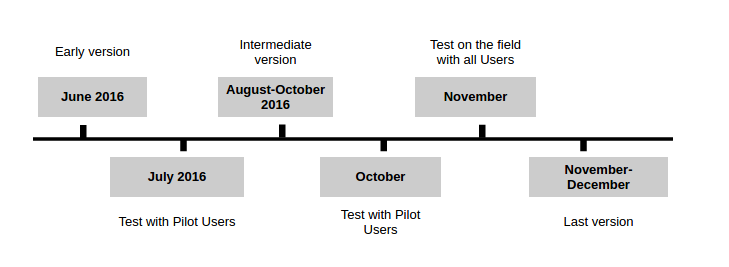
\includegraphics[scale=0.5]{TimeLine.png} 
\caption{An overview of the timeline of the project}
\end{figure}


\section{Analysis with inspection methods and Tests with users}
These are methods to try to judge the application (if necessary more than one time) during the developing process. There are two different situation:

\begin{enumerate}

% 1
\item For that regards the inspection analysis we must note that the evaluator is only one, and he is also the developer. This can be a big limit because only one evaluator can find only a little part of the problems. Also, the assessor is the same person who is designing this interface; accepted that this kind of analysis will not be the best source of feedbacks about the application a good solution is to check the various parts of the application against the Nielsen principles in the meanwhile these parts are designed and created.

%2
\item For that regards the opportunity to test the application with the users instead the situation is excellent: we have a good amount of users, they are very accessible, their roles and characteristics are known and precisely defined, and we also have two super-users that can help driving the design process into the good direction (actually these users play a role that can be considered also a designer-customer role). At this point we can hope that the confrontation with the users is the best available source for new ideas and a way to find and understand problems.    

\end{enumerate}

We note that in this project the evaluation is mostly a "formative evaluation", and only in the last stage it becomes a "summary evaluation". This is because the confrontation with the users is the only intelligent way to understand in which direction work and to enter in their "domain". So the formative evaluation, both from the two super-users, and from the generic users, is probably the most important source of requisites and solutions.   

\section{Prototyping and mock-up}
In this project the use of mock-ups is an example of interactive mock-ups. All the mock-ups are produced directly with HTML-scss-javascript-Php so they are real part of the websites. In that cases they are mock-ups only because some functionalities related to gAn on the back-end are still not implemented at the moment of the creation of the front-end. In the final version almost all of the website is real and working. Does it means that the application is ready and finished? No, it doesn't: still the server is not working properly (we are pretty sure that we can solve formatting it and re-distributing some of the applications installed on that server on other machines) and only some of the analysis prepared for the software are ready (the output of the others, is actually, a mock-up). The aim of the decision of working with interactive mock-ups directly produced by web programming technologies is related to the fact that the developer is very inexperienced using mock-up software but quite used to work with web development, so working directly with the web development seems to be a quite fast way, and the interactive mock-ups are perfect to be used to show the progresses of the application to the super-users.
Often the problem of interactive mock-ups are that the developer is reluctant to modify them.. and it is true, but in this case the continuous modification of the application through the different development stages is very important to arrive progressively to a good solution able to meet the users needs. In fact we can see that the system in the different stages is very different, actually at each iteration the production of the website re-started almost from zero. 

\section{Ambiguities and doubts}
Every time in the design process there is a doubt related to a requirement the adopted solution is to ask directly to the users what solution to implement. This means ask before to the super users (for motivations related to their role of supervisors of this project) end possibly observe the behavior of general 
users during the tests.

\section{How the various stages are presented}
According to this division in three main stages we can organize the following chapters in this way:
each chapter is related to a stage of the development: Early stage (  \ref{Chapter3} ), intermediate stage ( \ref{Chapter4} ) and final stage ( \ref{Chapter5} ). Also there is a chapter able to describe the tests with the users, so it is strictly related to the chapter 5: it is chapter 6 ( \ref{Chapter6} ).
For each of the three stages of the development this document will explain:

\begin {enumerate}

\item
The requirements of the web interface.

\item
The functional analysis of the requirements through some expected scenarios

\item
The resulting prototyping (and implementation)  

\end {enumerate} 



 